\documentclass[sigconf]{acmart}

%% Using the option "anonymous" will produce "Anonymous Author(s)"
%% for double-anonymized review. Upon acceptance, remove this option
%% and set the authors' names and affiliations using the corresponding
%% commands.

%% CBSoft uses an ACM-like format without the ACM Reference block.
%% The following warning from acmart can be safely ignored:
%% "ACM reference format is mandatory for papers over one page."
\settopmatter{printacmref=false}
\renewcommand\footnotetextcopyrightpermission[1]{} % removes footnote with conference information in first column

%% CBSoft uses an ACM-like format without a copyright note.
\setcopyright{none}

%% These commands are for a PROCEEDINGS abstract or paper.
\acmConference[SBES 2026]{40th Brazilian Symposium on Software Engineering}{September 8–11, 2026}{São Paulo, SP, Brazil}

% CBSoft uses an ACM-like format without CCS Concepts.
% The following warning from acmart can be safely ignored:
% "CCS concepts are mandatory for papers over two pages."

%% \BibTeX command to typeset BibTeX logo in the docs
\AtBeginDocument{
    \providecommand\BibTeX{{Bib\TeX}}
}

%% Only for papers written in PORTUGUESE: 
%% comment out the following three lines
%\renewcommand\abstractname{Resumo}
%\renewcommand\keywordsname{Palavras-chave}
%\renewcommand\refname{Referências}

%% end of the preamble, start of the body of the document source.


% ------------------------------------------------------------
% Authors: please make sure to read the checklist comments
% provided at the end of this document before submission.
% ------------------------------------------------------------
\begin{document}

%% The "title" command has an optional parameter,
%% allowing the author to define a "short title" to be used on the page 
%% headers.
\title{The Name of the Title Is Hope}

%% The "author" command and its associated commands are used to define
%% the authors and their affiliations.
%% Of note is the shared affiliation of the first two authors, and the
%% "authornote" and "authornotemark" commands
%% used to denote shared contribution to the research.
\author{FirstName Surname1stAutor}
\affiliation{
  \institution{DepartmentName, Institution/UniversityName}
  \city{City}
  \country{Country}
}
\email{email@email.com}

\author{FirstName Surname}
\affiliation{
  \institution{DepartmentName, Institution/UniversityName}
  \city{City}
  \country{Country}
}
\email{email@email.com}

\author{FirstName Surname}
\affiliation{
  \institution{DepartmentName, Institution/UniversityName}
  \city{City}
  \country{Country}
}
\email{email@email.com}

\author{FirstName Surname}
\affiliation{
  \institution{DepartmentName, Institution/UniversityName}
  \city{City}
  \country{Country}
}
\email{email@email.com}

\author{FirstName Surname}
\affiliation{
  \institution{DepartmentName, Institution/UniversityName}
  \city{City}
  \country{Country}
}
\email{email@email.com}

\author{FirstName Surname}
\affiliation{
  \institution{DepartmentName, Institution/UniversityName}
  \city{City}
  \country{Country}
}
\email{email@email.com}

\author{FirstName Surname}
\affiliation{
  \institution{DepartmentName, Institution/UniversityName}
  \city{City}
  \country{Country}
}
\email{email@email.com}

\author{FirstName Surname}
\affiliation{
  \institution{DepartmentName, Institution/UniversityName}
  \city{City}
  \country{Country}
}
\email{email@email.com}

\author{FirstName Surname}
\affiliation{
  \institution{DepartmentName, Institution/UniversityName}
  \city{City}
  \country{Country}
}
\email{email@email.com}

%% By default, the full list of authors will be used on the page
%% headers. This list is often too long and will overlap
%% other information printed in the page headers. 
%% This command allows the author to define a more concise list
%% of authors' names for this purpose.
\renewcommand{\shortauthors}{Surname1stAuthor et al.}
\renewcommand{\shorttitle}{The Name of the Title Is Hope}

%% The abstract is a short summary of the work the paper presents.
\begin{abstract}

\end{abstract}

%% Keywords. The author(s) should pick words that accurately describe
%% the presented work. Separate the keywords with commas.
\keywords{Do, Not, Use, This, Code, Put, the, Correct, Terms, for, Your, Paper}

%% This command processes the author, affiliation, and title
%% information and builds the first part of the formatted document.
%% "frenchspacing" avoids an additional space after a period at the end of a sentence.
\frenchspacing
\maketitle

\section{Introduction}

The article template adopted for CBSoft \footnote{CBSoft website: \url{
https://cbsoft.sbc.org.br/}} is an ACM-like version derived from the original ACM consolidated template. It preserves the visual identity and structural organization of the \verb|acmart| class, while adapting its elements to comply with the formatting guidelines and editorial context of CBSoft and the Brazilian Computer Society (SBC).

Originally introduced by ACM in 2017, the consolidated template was designed to provide a consistent \LaTeX\ style across a wide range of publications and to incorporate accessibility and metadata-extraction features to support digital libraries. In this adapted version, the principles are maintained, while ACM-specific submission requirements have been removed or adjusted to align with the CBSoft publication process.

\section{Template Overview}

As noted in the introduction, this ACM-like template for CBSoft is derived from the original \verb|acmart| document class and can be used to prepare different types of submissions accepted by the conference, including full research papers, short papers, tool papers, and other publication formats defined by the CBSoft symposia and workshops. The template supports the main stages of the publication process, from review versions to final camera-ready copies, by selecting appropriate template styles and parameters.

This document presents the main features of the adapted document class and explains how to use its elements in accordance with the CBSoft formatting guidelines. Since this template is based on the ACM consolidated format, authors familiar with the original \verb|acmart| class will find its structure and commands largely preserved, while ACM-specific requirements have been removed or adjusted to fit the CBSoft publication process.

\subsection{Template Parameters}

There are a number of {\itshape template parameters}
which modify some part of the applied template style. A complete list
of these parameters can be found in the {\itshape \LaTeX\ User's Guide.}

Frequently-used parameters, or combinations of parameters, include:
\begin{itemize}
\item {\texttt{anonymous,review}}: Suitable for a double-anonymized conference submission. It anonymizes the work and includes line numbers.
\item{\texttt{authorversion}}: Produces a version of the work suitable for posting by the author.
\item{\texttt{screen}}: Produces colored hyperlinks.
\end{itemize}


\section{Modifications}

Modifying the template, including but not limited to adjusting
margins, typeface sizes, line spacing, paragraph and list definitions,
and the use of the \verb|\vspace| command to manually adjust the
vertical spacing between elements of your work, \textbf{is not allowed.}

\textbf{Your document will be returned to you for revision if modifications are discovered.}


\section{Typefaces}

The \verb|acmart| document class requires the use of the Libertine typeface family. Your \TeX\ installation should include this set of packages. Please do not replace it with other typefaces. The \verb|lmodern| and  \verb|ltimes| packages should not be used, as they will override the built-in typeface families.

\section{Title Information}

The title of your work should use capital letters appropriately --\url{https://capitalizemytitle.com/} has useful rules for capitalization. Use the {\verb|title|} command to define the title of your work. If your work has a subtitle, define it with the {\verb|subtitle|} command. Do not insert line breaks in your title.

If your title is lengthy, you must define a short version to be used in the page headers to prevent overlapping text. The \verb|title| command has a ``short title'' parameter:
\begin{verbatim}
  \title[short title]{full title}
\end{verbatim}

\section{Authors and Affiliations}

Each author must be defined separately for accurate metadata
identification. As an exception, multiple authors may share one
affiliation. Authors' names should not be abbreviated; use full first
names wherever possible. Inclusion of e-mail addresses for all authors is mandatory and must follow the font style defined in the template.

Immediately below the title, each author must be declared using the following format:

\begin{center}
\begin{minipage}{\columnwidth}
\small
\begin{verbatim}
\author{FirstName Surname}
\affiliation{
  \institution{Department Name, Institution/University Name}
  \city{City}
  \country{Country}
}
\email{email@email.com}
\end{verbatim}
\end{minipage}
\end{center}

Grouping authors' names or e-mail addresses, or providing an ``e-mail
alias,'' as shown below, is not acceptable:
\begin{verbatim}
\author{Brooke Aster, David Mehldau}
\email{dave,judy,steve@university.edu}
\email{firstname.lastname@phillips.org}
\end{verbatim}

For papers with multiple authors, the surnames of the authors must be included in the page headers. The list of author names shown in the header must not exceed the column width. Therefore, only the surnames should be used, preferably in the form ``Surname et al.'' when appropriate. This shortened list must be explicitly defined using the following command, placed immediately after the last \verb|\author| declaration:

\begin{verbatim}
\renewcommand{\shortauthors}{Surname1stAuthor et al.}
\end{verbatim}

Omitting this command may cause the full list of authors to be automatically used in the page headers, which can lead to text overlap and layout issues.

The \verb|authornote| and \verb|authornotemark| commands allow a note
to apply to multiple authors. For example, if the first two authors
of an article contributed equally to the work.

Before submitting the camera-ready version, authors must verify the following:
\begin{itemize}
  \item All authors are declared individually using the required format.
  \item All e-mail addresses have been correctly included.
  \item The font used for e-mail addresses is consistent with the template.
  \item The shortened author list defined by \verb|\shortauthors| contains only surnames and fits within the column width of the header.
\end{itemize}

\section{Sectioning Commands}

Your work should use standard \LaTeX\ sectioning commands:
\verb|\section|, \verb|\subsection|, \verb|\subsubsection|,
\verb|\paragraph|, and \verb|\subparagraph|. The sectioning levels up to
\verb|\subsubsection| should be numbered; do not remove the numbering
from the commands.

All numbered section and subsection titles must follow the same capitalization style: the first letter of each word in the title must be capitalized (Title Case).

Simulating a sectioning command by setting the first word or words of a paragraph in boldface or italicized text is {\bfseries not allowed.}

Below are examples of sectioning commands:

\subsection{Subsection}
\label{sec:subsection}

This is a subsection.

\subsubsection{Subsubsection}
\label{sec:subsubsection}

This is a subsubsection.

\paragraph{Paragraph}

This is a paragraph.

\subparagraph{Subparagraph}

This is a subparagraph.

\section{Tables}

This ACM-like CBSoft template, based on the \verb|acmart| document class, includes the \verb|booktabs| package (\url{https://ctan.org/pkg/booktabs})- for preparing high-quality tables.

Table captions are placed \textbf{above} the table.

Because tables cannot be split across pages, the best placement is typically at the top of the page nearest their initial citation. To ensure this proper ``floating'' placement of tables, use the \texttt{table} environment to enclose the table's contents and the table caption. The contents of the table must be placed in the \texttt{tabular} environment to ensure proper row and column alignment. Do not use horizontal lines between rows with \texttt{hline}, except for the table header and marking its end. Do not use vertical lines between columns in any case.

Immediately following this sentence is the point at which Table~\ref{tab:freq} is included in the input file; compare the placement of the table here with the table in the printed output of this document.

\begin{table}
  \caption{Frequency of special characters}
  \label{tab:freq}
  \begin{tabular}{ccl}
    \toprule
    Non-English or Math & Frequency   & Comments\\
    \midrule
    \O                  & 1 in 1,000  & For Swedish names\\
    $\pi$               & 1 in 5      & Common in math\\
    \$                  & 4 in 5      & Used in business\\
    $\Psi^2_1$          & 1 in 40,000 & Unexplained usage\\
  \bottomrule
\end{tabular}
\end{table}

To set a wider table, which takes up the whole width of the page's live area, use the \texttt{table*} environment to enclose the table's contents and the table caption. As with a single-column table, this wide table will ``float'' to a location deemed more desirable. Immediately following this sentence is the point at which Table~\ref{tab:commands} is included in the input file. Once again, it is instructive to compare the placement of the table here with the table in the printed output of this document.

\begin{table*}
  \caption{Some typical commands}
  \label{tab:commands}
  \begin{tabular}{ccl}
    \toprule
    Command                     & A Number  & Comments\\
    \midrule
    \texttt{{\char'134}author}  & 100       & Author\\
    \texttt{{\char'134}table}   & 300       & For tables\\
    \texttt{{\char'134}table*}  & 400       & For wider tables\\
    \bottomrule
  \end{tabular}
\end{table*}

Always use \texttt{midrule} to separate table header rows from data rows, and use it only for this purpose. This enables assistive technologies to recognize table headers and support their users in navigating tables more easily.

\section{Math Equations}
You may want to display math equations in three distinct styles: inline, numbered, or non-numbered display. Each of the three is discussed in the next sections.

\subsection{Inline (In-text) Equations}
A formula that appears in the running text is called an inline or in-text formula. It is produced by the \texttt{math} environment, which can be invoked with the usual \texttt{{\char'134}begin\,\ldots{\char'134}end} construction or with the short form \texttt{\$\,\ldots\$}. You can use any of the symbols and structures, from $\alpha$ to $\omega$, available in \LaTeX~\cite{Lamport:LaTeX}; this section will simply show a few examples of in-text equations in context. This is an equation in in-line math style:

\begin{math}
  \lim_{n\rightarrow \infty}x=0
\end{math},

It looks slightly different when set in display style (see next section).

\subsection{Display Equations}
A numbered display equation, set off by vertical space from the text and centered horizontally, is produced by the \texttt{equation} environment. An unnumbered display equation is produced by the \texttt{displaymath} environment.

Once again, in either environment, you can use any of the symbols and structures available in \LaTeX\@; this section gives just a couple of examples of display equations in context. First, consider the equation, shown as an inline equation above:
\begin{equation}
  \lim_{n\rightarrow \infty}x=0
\end{equation}

Notice how it is formatted somewhat differently in the \texttt{displaymath} environment. Now, we will enter an unnumbered equation:
\begin{displaymath}
  \sum_{i=0}^{\infty} x + 1
\end{displaymath}

And this is another numbered equation:
\begin{equation}
  \sum_{i=0}^{\infty}x_i=\int_{0}^{\pi+2} f
\end{equation}

\section{Figures}

The \verb|figure| environment should be used for figures. One or more images can be placed within a figure. If your figure contains third-party material, you must clearly identify it as such, as shown in the example below.

\begin{figure}[ht]
  \centering
  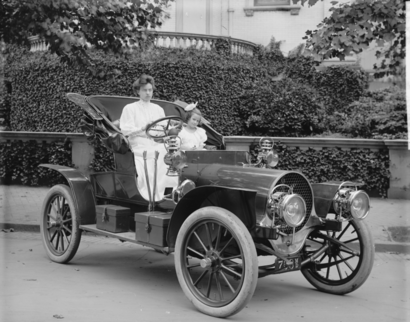
\includegraphics[width=\linewidth]{sample-franklin}
  \caption{1907 Franklin Model D roadster. Photograph by Harris \& Ewing, Inc. [Public domain], via Wikimedia Commons. (\url{https://goo.gl/VLCRBB}).}
  \Description{A woman and a girl in white dresses sit in an open car.}
\end{figure}

Figure captions are placed \textbf{below} the figure.

Every figure should also have a figure description with the \texttt{\Description} command unless it is purely
decorative. These descriptions convey what is s in the image to someone
who cannot see it. They are also used by search engine crawlers for
indexing images, and when images cannot be loaded.


\section{Citations and Bibliographies}

The use of \BibTeX\ for the preparation and formatting of one's references is strongly recommended. Authors' names should be complete. Use full first names (``Donald E. Knuth'') instead of initials (``D. E. Knuth''), and the identifying features of a reference must be included: title, year, volume, number, pages, article DOI, etc.

The bibliography is included in your source document with these two
commands, placed just before the \verb|\end{document}| command:
\begin{verbatim}
  \bibliographystyle{ACM-Reference-Format}
  \bibliography{bibfile}
\end{verbatim}

\verb|bibfile| is the \BibTeX\ filename without the \verb|.bib| suffix.

Citations and references are numbered by default. Some examples:
\begin{itemize}
\item A paginated journal article \cite{Abril07}
\item An enumerated journal article \cite{Cohen07}
\item A reference to an entire issue \cite{JCohen96}
\item A monograph (whole book) \cite{Kosiur01}
\item A monograph/whole book in a series \cite{Harel79}
\item A divisible book such as an anthology or compilation \cite{Editor00}
\item A divisible book (series not included since no volume number is given) \cite{Editor00a}
\item A chapter in a divisible book \cite{Spector90}
\item A chapter in a divisible book in a series \cite{Douglass98}
\item A multi-volume work as a book \cite{Knuth97}
\item Paginated proceedings articles \cite{Andler79, Hagerup1993}
\item A proceedings article with all possible elements \cite{Smith10}
\item An enumerated proceedings article \cite{VanGundy07}
\item An informally published work \cite{Harel78}
\item Preprints \cite{Bornmann2019, AnzarootPBM14}
\item A doctoral dissertation \cite{Clarkson85}
\item A master's thesis \cite{anisi03}
\item Online documents / World Wide Web resources \cite{Thornburg01, Ablamowicz07, Poker06}
\item Video games (Case 1) \cite{Obama08}
\item Video games (Case 2) \cite{Novak03, Lee05}
\item A patent (Case 3) \cite{JoeScientist001}
\item Work accepted for publication \cite{rous08}
\item `YYYYb' test for prolific author \cite{SaeediMEJ10, SaeediJETC10}
\item Citations containing duplicate DOI and URLs (e.g., some SIAM articles) \cite{Kirschmer:2010:AEI:1958016.1958018}
\item Multi-volume works as books \cite{MR781536, MR781537}
\item A presentation \cite{Reiser2014}
\item An article under review \cite{Baggett2025}
\item Citations with DOIs \cite{2004:ITE:1009386.1010128, Kirschmer:2010:AEI:1958016.1958018}
\item Online citations \cite{TUGInstmem, Thornburg01, CTANacmart}
\item Artifacts \cite{R, UMassCitations}
\end{itemize}


\section{Recomme that demonstratependices}

If your work needs an appendix, add it before the \verb|\end{document}| command at the conclusion of your source document.

Start the appendix with the \verb|appendix| command:
\begin{verbatim}
  \appendix
\end{verbatim}

In the appendix, sections are lettered rather than numbered. This document has two appendices that demonstrate the section and subsection identification method.

\section{Conclusion and Future Work}
<text included by the authors>

\section*{Artifact Availability}
This section must be included immediately after the Conclusion and before the Acknowledgments section. It must not be numbered and must be titled exactly as \textbf{Artifact Availability}.

If the paper provides research artifacts (such as datasets, source code, scripts, models, or experimental packages), the authors must describe what is available, where it can be accessed, and under which license or usage conditions.

If no artifacts are available, this section must still be included, explicitly stating that no artifacts are provided.

For papers written in Portuguese, this section must be titled
\textbf{Disponibilidade de Artefatos}.

\section*{Acknowledgements}
<text included by the authors>

%% The next two lines define the bibliography style to be used, and
%% the bibliography file.
\bibliographystyle{ACM-Reference-Format}
\bibliography{sample-base}

%% If your work has appendices, this is the place to put them
\appendix

\section{Appendix Example 1}

\subsection{Part One}
Lorem ipsum dolor sit amet, consectetur adipiscing elit. Morbi malesuada, quam in pulvinar varius, metus nunc fermentum urna, id sollicitudin purus odio sit amet enim. Aliquam ullamcorper eu ipsum vel mollis. Curabitur quis dictum nisl. Phasellus vel semper risus, et lacinia dolor. Integer ultricies commodo sem nec semper.

\subsection{Part Two}
Etiam commodo feugiat nisl pulvinar pellentesque. Etiam auctor sodales ligula, non varius nibh pulvinar semper. Suspendisse nec lectus non ipsum convallis congue hendrerit vitae sapien. Donec at laoreet eros. Vivamus non purus placerat, scelerisque diam eu, cursus ante. Etiam aliquam tortor auctor efficitur mattis.

\section{Appendix Example 2}
Nam id fermentum dui. Suspendisse sagittis tortor a nulla mollis, in pulvinar ex pretium. Sed interdum orci quis metus euismod, et sagittis enim maximus. Vestibulum gravida massa ut felis suscipit congue. Quisque mattis elit a risus ultrices commodo venenatis eget dui. Etiam sagittis eleifend elementum.

Nam interdum magna at lectus dignissim, ac dignissim lorem rhoncus. Maecenas eu arcu ac neque placerat aliquam. Nunc pulvinar massa et mattis lacinia.

\end{document}

% ============================================================
% CBSoft ACM-like Template – Author Checklist
% ============================================================
%
% 1. Remove CCS Concepts
%    - Remove the CCSXML block and \ccsdesc commands.
%
% 2. Remove ACM footer
%    Use the command \renewcommand\footnotetextcopyrightpermission[1]{}
%
% 3. Remove ACM Reference Format
%    Use the commands \setcopyright{none} and 
%    \settopmatter{printacmref=false}
%
% 4. Short title must not exceed column width
%    Use the command 
%    \renewcommand{\shorttitle}{The Name of the Title Is Hope}
%
% 5. Include authors' surnames in the page headers (even pages)
%    - The author names in the page header (at the top of the page)
%      must not exceed the column width
%    - This list must contain only the authors' surnames
%    - Suggestion: use "Surname et al." for more than two authors with the
%      command \renewcommand{\shortauthors}{Surname1stAuthor et al.}
%
% 6. Author format below title:
%    \author{FirstName Surname}
%    \affiliation{
%      \institution{Department, Institution}
%      \city{City}
%      \country{Country}}
%    \email{email@email.com}
%
% 7. Verify all author emails are included
%    - Check font consistency
%
% 8. All numbered section and subsection titles must follow the same
%    capitalization style: the first letter of each word in the title 
%    must be capitalized (Title Case).
%
% 9. Artifact Availability (check CFP)
%    - Not numbered -- use \section*{Artifact Availability}
%    - Placed after Conclusion and before Acknowledgments
%    - In Portuguese, use \section*{Disponibilidade de Artefatos}
%
% 10. Abstract
%     - Single paragraph
%     - Papers written in Portuguese must use "Resumo" instead of "Abstract"
%       with the command \renewcommand\abstractname{Resumo}
%
% 11. Keywords
%     - Comma-separated, first letter capitalized
%     - Papers written in Portuguese must use "Palavras-chave" instead of
%       "Keywords" with the command 
%       \renewcommand\keywordsname{Palavras-chave}
%
% 12. References
%     - Not numbered -- already enforced by the template
%     - Papers written in Portuguese must use "Referências" instead of
%       "References" with the command \renewcommand\refname{Referências}
%
% 13. Acknowledgements
%     - Optional section
%     - Not numbered -- use \section*{Acknowledgements}
%     - In Portuguese, use \section*{Agradecimentos}
%
% 14. Remove received/revised/accepted dates
%
% 15. Figure captions must appear below figures
%
% 16. Verify the symposium name in the page header
%    - Use English, even if the paper is written in Portuguese
%    - Select the correct event according to the track
%    - Use Arabic ordinal numbers, not Roman
%
%    SBES (Research, Education, IIER, Tools, Industry)
%    \acmConference[SBES 2026]{40th Brazilian Symposium on Software Engineering}{September 8--11, 2026}{São Paulo, SP, Brazil}
%
%    SBLP
%    \acmConference[SBLP 2026]{30th Brazilian Symposium on Programming Languages}{September 8--11, 2026}{São Paulo, SP, Brazil}
%
%    SBCARS
%    \acmConference[SBCARS 2026]{20th Brazilian Symposium on Software Components, Architectures, and Reuse}{September 8--11, 2026}{São Paulo, SP, Brazil}
%
%    SAST
%    \acmConference[SAST 2026]{11st Brazilian Symposium on Systematic and Automated Software Testing}{September 8--11, 2026}{São Paulo, SP, Brazil}
%
%    Workshops
%    \acmConference[Workshop Acronym 2026]{Workshop Full Name}{Workshop Date}{São Paulo, SP, Brazil}
%
%
% 17. Remove colored author names, citations, and links
%
% 18. Camera-ready only:
%     Do not use the "review" or "anonymous" modes in the 
%     \documentclass command
%
% 19. SBES Tools Track papers must include a demo video link at the end of
%     the abstract
%     Example:
%     \begin{abstract}
%     <abstract text> \newline
%     \textbf{Demo video:} <video link>
%     \end{abstract}
%
% 20. SBES Industry Track papers must not include author biographies
%
% ============================================================

\endinput


